% ----------------------------------------------------------------------
%                   LATEX TEMPLATE FOR PhD THESIS
% ----------------------------------------------------------------------

% based on Harish Bhanderi's PhD/MPhil template, then Uni Cambridge
% http://www-h.eng.cam.ac.uk/help/tpl/textprocessing/ThesisStyle/
% corrected and extended in 2007 by Jakob Suckale, then MPI-CBG PhD programme
% and made available through OpenWetWare.org - the free biology wiki


%: Style file for Latex
% Most style definitions are in the external file PhDthesisPSnPDF.
% In this template package, it can be found in ./Latex/Classes/
\documentclass[twoside,11pt]{Latex/Classes/PhDthesisPSnPDF}

%: Macro file for Latex
% Macros help you summarise frequently repeated Latex commands.
% Here, they are placed in an external file /Latex/Macros/MacroFile1.tex
% An macro that you may use frequently is the figuremacro (see introduction.tex)
% This file contains macros that can be called up from connected TeX files
% It helps to summarise repeated code, e.g. figure insertion (see below).

% produce an unit vector
\newcommand{\unitvector}[1]{\ensuremath{\hat{\mathbf{#1}}}}
% produce the normal vector
\newcommand{\normal}{\ensuremath{\hat{\mathbf{n}}}}
%\newcommand{\unitvector}[2]{\ensuremath{\hat{\mathbf{#1}}_{#2}}}
\newcommand{\point}[1]{\ensuremath{\mathbf{#1}}}
\newcommand{\pointi}[2]{\ensuremath{\mathbf{#1}_{#2}}}
%put figure and table in multicols environment.
\makeatletter
\newenvironment{tableInMulticols}
  {\def\@captype{table}}
  {}

\newenvironment{figureInMulticols}
  {\def\@captype{figure}}
  {}
\makeatother

% insert a centered figure with caption and description
% parameters 1:filename, 2:title, 3:description and label
\newcommand{\figuremacro}[3]{
	\begin{figure}[htbp]
		\centering
		\includegraphics[width=1\textwidth]{#1}
		\caption[#2]{\textbf{#2} - #3}
		\label{#1}
	\end{figure}
}

% insert a centered figure with caption and description AND WIDTH
% parameters 1:filename, 2:label, 3:caption, 4: textwidth
% textwidth 1 means as text, 0.5 means half the width of the text
\newcommand{\figuremacroW}[4]{
	\begin{figure}[htbp]
		\centering
		\includegraphics[width=#4\textwidth]{#1}
		\caption{#3}
		\label{#2}
	\end{figure}
}

% inserts a figure with wrapped around text; only suitable for NARROW figs
% o is for outside on a double paged document; others: l, r, i(inside)
% text and figure will each be half of the document width
% note: long captions often crash with adjacent content; take care
% in general: above 2 macro produce more reliable layout
\newcommand{\figuremacroN}[3]{
	\begin{wrapfigure}{o}{0.5\textwidth}
		\centering
		\includegraphics[width=0.48\textwidth]{#1}
		\caption[#2]{{\small\textbf{#2} - #3}}
		\label{#1}
	\end{wrapfigure}
}

% predefined commands by Harish
\newcommand{\PdfPsText}[2]{
  \ifpdf
     #1
  \else
     #2
  \fi
}

\newcommand{\IncludeGraphicsH}[3]{
  \PdfPsText{\includegraphics[height=#2]{#1}}{\includegraphics[bb = #3, height=#2]{#1}}
}

\newcommand{\IncludeGraphicsW}[3]{
  \PdfPsText{\includegraphics[width=#2]{#1}}{\includegraphics[bb = #3, width=#2]{#1}}
}

\newcommand{\InsertFig}[3]{
  \begin{figure}[!htbp]
    \begin{center}
      \leavevmode
      #1
      \caption{#2}
      \label{#3}
    \end{center}
  \end{figure}
}


%%% Local Variables:
%%% mode: latex
%%% TeX-master: "~/Documents/LaTeX/CUEDThesisPSnPDF/thesis"
%%% End:


\DeclareMathAlphabet{\mathcal}{OMS}{cmsy}{m}{n}

%glossary ralated code
\usepackage[toc]{glossaries}
\renewcommand*{\glossaryentrynumbers}[1]{}
%\setlength{\glsdescwidth}{0.8\linewidth}
\makeglossaries

\glossarystyle{list}
\renewcommand*{\glsgroupskip}{}

\addbibresource[]{bibliography.bib}


% this file is called up by thesis.tex
% content in this file will be fed into the main document

% 1 = Entry name, e.g. abbreviation; 2 = Explanation
% You can place all explanations in this separate file or declare them in the middle of the text. Either way they will be collected in the glossary.

% required to print nomenclature name to page header
\newacronym{SLAM}{SLAM}{Simultaneous Localization And Mapping}
\newacronym{LRF}{LRF}{Laser Range Finder}
\newacronym{aLRF}{aLRF}{actuated Laser Range Finder}
\newacronym{NBV}{NBV}{Next Best Viewpoint}
\newacronym{FoV}{FoV}{Field of View}
\newacronym{ToF}{ToF}{Time of Flight}
%\newacronym{NNS}{NNS}{Nearest Neighbor Search}
\newacronym{EGI}{EGI}{Extended Gaussian Image}
%\newacronym{PCA}{PCA}{Principal Component Analysis}
\newacronym{MSE}{MSE}{Mean Square Error}
\newacronym{ICP}{ICP}{Iterative Closest Point}
\newacronym{NDT}{NDT}{Normal Distributions Transform}
\newacronym{3D-NDT}{3D-NDT}{Three-Dimensional Normal Distributions Transform}
\newacronym{MUMC}{MUMC}{Minimum Uncertainty Maximum Consensus}
\newacronym{IMU}{IMU}{Inertial Measurement Units}
\newacronym{GNSS}{GNSS}{Global Navigation Satellite Systems}
%\newacronym{EKF}{EKF}{Extended Kalman Filter}
%\newacronym{MLS}{MLS}{Multi-Level Surface}
\newacronym{PDF}{PDF}{Probability Density Functions}
%\newacronym{MLE}{MLE}{Maximum-Likelihood Estimation}
%\newacronym{P2D}{P2D}{Point-to-Distribution}
%\newacronym{FPFH}{FPFH}{Fast Point Feature Histograms}
%\newacronym{DIFT}{DIFT}{Depth-interpolated Image FeaTures}
\newacronym{RANSAC}{RANSAC}{RANdom SAmple Consensus}
\newacronym{SVM}{SVM}{Support Vector Machine}
\newacronym{PTU}{PTU}{Pan-Tilt Unit}
\newacronym{FILO}{FILO}{First-In-Last-Out}


%: ----------------------------------------------------------------------
%:                  TITLE PAGE: name, degree,..
% ----------------------------------------------------------------------
\ifpdf
    \pdfinfo { /Title  (PhD Thesis)
               /Creator (TeX)
               /Producer (pdfTeX)
               /Author (Benjamin Adler adler@informatik.uni-hamburg.de)
               /CreationDate (D:20140120)  %format D:YYYYMMDDhhmmss
               /ModDate (D:20140502)
               /Subject (robotics)
               /Keywords (Autonomous Robotics, Exploration, Mapping, SLAM) }
    \pdfcatalog { /PageMode (/UseOutlines)
                  /OpenAction (fitbh)  }
\fi

% ----------------------------------------------------------------------

% turn of those nasty overfull and underfull hboxes
\hbadness=10000
\hfuzz=50pt
%: --------------------------------------------------------------
%:                  FRONT MATTER: dedications, abstract,..
% --------------------------------------------------------------
%\makeglossaries
\begin{document}
% sets line spacing
\renewcommand\baselinestretch{1.0}
\baselineskip=14pt plus1pt

%: ----------------------- generate cover page ------------------------

\maketitle  % command to print the title page with above variables

%: ----------------------- tie in front matter ------------------------
%\frontmatter
\reviewers
%% Thesis Dedictation ---------------------------------------------------

\begin{dedication} %this creates the heading for the dedication page

To my family...

\end{dedication}

% ----------------------------------------------------------------------
%\phantomsection
\chapter*{Change list}
\markboth{\MakeUppercase{Change list}}{}
\addcontentsline{toc}{chapter}{Change list}

\begin{itemize}
 \item Figure 3.2(b), the horizontal field of view has been corrected to 360 degrees.
 \item Algorithm 4.4, line 1, duplicate of Q <-- emptyset.
\end{itemize}
% Thesis Acknowledgements ------------------------------------------------
\phantomsection
\chapter*{Acknowledgements}
\markboth{\MakeUppercase{Acknowledgements}}{}
\addcontentsline{toc}{chapter}{Acknowledgements}

\if0
Doing a PhD was a long and exciting journey, which would not be possible without the help and support of many people. First of all I am most grateful to my supervisor Prof. Dr. Jianwei Zhang for giving me the opportunity to pursue a PhD at the University of Hamburg and providing me such a good and liberal academic environment. 

Next, I would like to extend my thanks to my daily supervisor and good friend Prof. Dr. Houxiang Zhang, whose support was always there for both technical and personal problems, not only in the first two years of my study when he was in Hamburg, but also for the second two years after he moved to {\AA}lesund. His constructive criticism helped focus my ideas and his constant encouragement kept me going in spite of many stumbling blocks on the road.    

Writing a dissertation is no easy task, but the same can be said of reviewing it. I would like to thank all the people who helped by reviewing parts of this work, especially my external reviewers --- Prof. Dr. Reinhard Koch and Dr. Peer Stelldinger. 

%I have to say, without your encouragement, I was almost going to drop when the traffic accident came to me while I had been ill for a long time. 

All the members of our TAMS group are greatly acknowledged, the time spent with you was wonderful. I own a great deal to Tatjana (Lu) Tetsis, thank you for helping me so much during the past time. My sincere thanks also go to Benjamin Adler for always being excited about my problems and ideas, always sharing his ideas with me, and the engaging discussions we had during and after work. 

I am grateful to my former colleagues from NuBot, Huimin Lu, Xiangke Wang, and Shaowu Yang are especially acknowledged, thanks a lot for valuable comments and suggestions on my conference and journal papers, as well as this dissertation. 

%I am thankful to all the people who helped by reviewing this work, they are Dr. Norman Hendrich, Shaowu Yang, Benjamin Adler, Weiwei Kong, and Jie Liang; especially my external reviewers --- Prof. Dr. Reinhard Koch and Dr. Peer Stelldinger.   

Being away from my family was not easy, however, many friends from Hamburg and other places provided another family away from home. I own special thanks to all of my friends. In this regard, Jianhua Zhang, Guoyuan Li, Gang Cheng, Bo Sun, and Weiwei Kong deserve special mention.

Finally, I would like to thank the people closest to me for their love and support --- my parents and brother, my girl friend Fang, especially to my little nephew who brings a lot of happy moments.  
\fi
% ------------------------------------------------------------------------

\vspace*{5mm}

\hfill Benjamin Adler

\hfill Hamburg, May 2014

\phantomsection
\chapter*{Abstract}
\markboth{\MakeUppercase{Abstract}}{}
\addcontentsline{toc}{chapter}{Abstract}

This paper introduces a custom-built unmanned aerial vehicle, capable of autonomous exploration in urban environments. It consists of a multicopter, an inertial navigation system and two 2D laser range finders. In addition to a description of the hardware architecture and individual components being used, the authors also discuss challenges and problems that arose during its construction as well as optimizations and workarounds applied in the course of its development.

Also presented is the software architecture, with a focus on a novel algorithm capable of generating multiple next best views (NBVs), sorted by achievable information gain. Although being designed for application on airborne platforms in urban environments, it works directly on raw point clouds and thus can be used with any sensor generating spatial occupancy information (e.g. LIDAR, RGBD- or time-of-flight-cameras). To satisfy constraints introduced by real-time operation on UAVs, the algorithm is implemented on a highly parallel SIMD architecture and benchmarked using GPUs from multiple hardware generations, using data from real flights. It is also compared against the previous, CPU-based proof of concept.

As the underlying hardware imposes limitations with regards to memory access and concurrency, necessary data structures and further performance considerations are explained in detail.

Open-source code for this paper is available at http://www.github.com/benadler/octocopter/.
\phantomsection
\chapter*{Kurzfassung}
\markboth{\MakeUppercase{Kurzfassung}}{}
\addcontentsline{toc}{chapter}{Kurzfassung}

Die vorliegende Dissertation behandelt ...
%: ----------------------- contents ------------------------
\setcounter{secnumdepth}{3} % organisational level that receives a numbers
\setcounter{tocdepth}{3}    % print table of contents for level 3
\tableofcontents            % print the table of contents
\addtocontents{toc}{\protect{\pdfbookmark[0]{\contentsname}{toc}}}
% levels are: 0 - chapter, 1 - section, 2 - subsection, 3 - subsection
%: ----------------------- list of figures/tables ------------------------
\listoffigures	% print list of figures
\newpage\thispagestyle{empty}
\listoftables  % print list of tables
\newpage\thispagestyle{empty}

%\glsaddall
\printglossaries
\newpage\thispagestyle{empty}


\begin{multicols}{2} % \begin{multicols}{#columns}[header text][space]
\begin{footnotesize} % scriptsize(7) < footnotesize(8) < small (9) < normal (10)
\printnomenclature[1.5cm] % [] = distance between entry and description
\label{nom} % target name for links to glossary

\end{footnotesize}
\end{multicols}

%: --------------------------------------------------------------
%:                  MAIN DOCUMENT SECTION
% --------------------------------------------------------------

% the main text starts here with the introduction, 1st chapter,...
\mainmatter
%: ----------------------- subdocuments ------------------------
% Parts of the thesis are included below. Rename the files as required.
% But take care that the paths match. You can also change the order of appearance by moving the include commands.

%: ----------------------- introduction file header -----------------------
\chapter{Einleitung}
%\epigraph{Pommes sind lecker.}{Ben}
% the code below specifies where the figures are stored
\ifpdf
    \graphicspath{{1_introduction/figures/PNG/}{1_einleitung/figures/PDF/}{1_einleitung/figures/}}
\else
    \graphicspath{{1_einleitung/figures/EPS/}{1_einleitung/figures/}}
\fi

% ----------------------------------------------------------------------
%: ----------------------- introduction content -----------------------
% ----------------------------------------------------------------------


While robots ...

\begin{quote}
``It is not that difficult to build computers capable of playing chess or doing sums. Computers find it easy to do what we learned at school. But computers have a very hard time learning what children learn \textit{before} they start school: [...] navigating a backyard, recognizing a face; seeing.'' 
\end{quote}

\begin{itemize}
\item der erste Punkt
\item der zweite Punkt
\end{itemize}

\begin{enumerate}
\item der erste Punkt
\item der zweite Punkt
\end{enumerate}

\section{Motivation} % section headings are printed smaller than chapter names
\lettrine{H}{uman} beings have been dreaming to create intelligent \emph{robots} 

\subsection{Untergedängs}
tüdlötß
\subsubsection{unteruntergedaengs}
hehe

\paragraph{hahaha parapgrah}

\section{Outline}
\indent{The rest of this thesis is organized as follows: }

Chapter \ref{chapter:soa} 

\section{Research questions and contributions}
\label{sec:introduction:contributions}

\newpage\thispagestyle{empty}
\ifpdf
\graphicspath{{2_chronisch_obstruktive_lungenerkrankung/figures/PNG/}{2_chronisch_obstruktive_lungenerkrankung/figures/PDF/}{2_chronisch_obstruktive_lungenerkrankung/figures/}}
\else
    \graphicspath{{2_chronisch_obstruktive_lungenerkrankung/figures/EPS/}{2_chronisch_obstruktive_lungenerkrankung/figures/}}
\fi

\chapter{Chronisch obstruktive Lungenerkrankung (COPD)}
\label{chapter:copd}

Die Chronisch obstruktive Lungenerkrankung, auf englisch Chronic Obstructive Pulmonary Disease (COPD) genannt, ist trotz ihrer starken Verbreitung noch vielen Menschen nicht bekannt.
Bei der COPD handelt es sich um eine chronische Lungenkrankheit mit progredienter Atemwegsverengung; sie gilt als die häufigste Erkrankung der Atmungsorgane. COPD ist ein Sammelbegriff für die chronisch obstruktive Bronchitis und das Lungenemphysem, welche entweder einzeln oder gemeinsam auftreten \autocite[vgl.][153]{lorenz2009}.  Die COPD resultiert aus einer langfristigen Entzündung der Atemwege, welche durch ständige Belastung mit in erster Linie Zigarettenrauch, aber auch Umweltfaktoren, Staubpartikeln und giftigen Dämpfen entsteht. Ätiologisch wird davon ausgegangen, dass 80-90\% der COPD-Patienten die Erkrankung aufgrund von Nikotinabusus entwickelt haben; das sind in etwa 15\% der Zigarettenraucher\autocite[vgl.][154]{lorenz2009}. 

Als ein wichtiges Diagnosemerkmal gilt die Atemnot (Dispnoe), welche aus der Obstruktion der Bronchien resultiert. Diese wird durch drei Faktoren ausgelöst: 

\begin{enumerate}
\item Verkrampfung der Bronchialmuskulatur (Bronchospasmus)
\item Anschwellen der Schleimhaut in den Bronchien (Ödem)
\item Krankhaft erhöhte Schleimproduktion (Hyperkrinie) aufgrund einer dauerhaften Entzündung der Atemwege (chronische Bronchitis)
\end{enumerate}

Durch die Hyperkrenie werden die Zilien - kleine Flimmerhärchen in den Bronchien - immer mehr daran gehindert, Schadstoffe aus der Lunge hinaus zu befördern, da ihre Bewegungsfähigkeit eingeschränkt wird. Dieser Prozess führt über einen längeren Zeitraum zur Zerstörung der Flimmerhärchen und somit zu einem größeren Exazerbationsrisiko (siehe unten).
Die Luftnot tritt im Anfangsstadium nur unter Belastung auf, später auch im Ruhezustand \autocite[vgl.][6f.]{lorenz2009}. Die allgemeine Symptomatik umfasst morgendlichen Kopfschmerz, Gewichtsverlust, welcher auf verstärkte Atemarbeit und systemische Entzündungsreaktionen zurückzuführen ist, zunehmenden Leistungsabfall, Einflussstauung, Ödeme der unteren Extremitäten und weiter abnehmende Belastbarkeit aufgrund des s.g. Cor pulmonale (Lungenherz, s. weiter unten).
Eine chronisch obstruktive Lungenerkrankung liegt laut WHO-Definition dann vor, wenn sowohl Husten und Auswurf über wenigstens als 3 Monate in mindestens 2 aufeinander folgenden Jahren bestehen und somit als chronisch anzusehen sind, als auch andere Krankheiten wie z.B. Bronchiektasen, Staubbelastung, cystische Fibrose, Asthma, Fremdkörper u.a. im Vorfeld ausgeschlossen werden konnten \autocite[vgl.][71]{koehler2010}. 

%todo Grafik der Lunge als auch der Lungenbläschen

Das Lungenemphysem ist das Resultat länger andauernder Entzündungsreaktionen auf o.g. mögliche externe Partikel. Durch entzündliche Prozesse  werden die Zellwände in den Alveolen  (Lüngenbläschen, siehe Abbildung todo) zerstört. Hierfür sind Proteasen zuständig, die bei Eindringen von schädlichen Stoffen in die Lunge durch das Immunsystem freigesetzt werden. So genannte Antiproteasen können jedoch vor der Zerstörung der Alveolarwände schützen. Diese werden für normal körpereigen produziert; hierzu gehört u.a. das Alpha-1-Antitripsin. Einige Patienten leiden jedoch unter einem genetische bedingen Alpha-1-Antripsinmangel, wodurch ein erhöhtes Risiko für die Ausbildung eines Lungenemphysems besteht.
Das bedeutet, dass sich mit weiterbestehender Entzündung die Anzahl der für den Sauerstoff-Kohlendioxid-Austausch notwendigen Alveolen verringert und sich die Lufträume in der Lunge vergrößern. Dadurch wird nach und nach die Lungenelastizität eingeschränkt, was eine Überdehnung der Lunge (Hyperinlation) mit Minderdurchblutung und einem irreversiblen Schwund an Lungengewebe als auch eine Einschränkung der Atemfunktion nach sich zieht. Dies geschieht jedoch nicht nur durch die degenerativen Prozesse in einem Lungenlappen, sondern auch durch funktionelle Beeinträchtigung anderer umliegender, gesunder Lungenlappen aufgrund der partiellen Überblähung. Auch andere Organe können möglicherweise beschädigt werden. Denn bei Nichtbehandlung des Emphysems kommt es zu einer erhöhten Pumpleistung des Herzmuskels und so über längere Zeit zu einer Schädigung desselben, da dieser nun mehr Blut transportieren muss, um die Organe ausreichend mit Sauerstoff zu versorgen. Daher ist die Todesursache bei einem Lungenemphysem in den meisten Fällen ein Herzversagen und nicht, wie evtl. zuvor vermutet, Erstickung.

Bei Fortschreiten der COPD kommt es immer wieder zu Exazerbationen, das heißt zu akuten Verschlechterungen der alltäglichen Krankheitssymptome, was zu Symptomen wie Atemnot, Husten, vermehrter Sputummenge oder Fieber führen kann. Sie resultieren zu 60-70\% aus einer Infektion der Lunge oder nichtinfektiösen Ursachen wie akuter Luftverschmutzung oder Verschlechterung von Begleiterkrankungen und sollten daher zeitnah behandelt werden.

Das Auftreten der COPD nimmt mit dem Alter zu, dabei kommt es ab dem 50. Lebensjahr zu einem rapiden Anstieg der Prävalenz. Im siebten Dezennium ist die Spitze des Auftretens mit etwa 10\% bei Männern und ca. 5\% bei Frauen erreicht\autocite[vgl.][153]{lorenz2009}. Nach Köhler/Schönhofer/Voshaar sei Vorsicht geboten bei dem Einbezug von Statistiken in diesem Bereich, da die verfügbaren Daten zur Prävalenz der COPD sehr von dem untersuchten Kollektiv bzw. den Altersgruppen abhängen (2010: 72). Insgesamt gehen sie jedoch von folgenden Zahlen aus: Etwa 10\% der deutschen Bürger ab dem 40. Lebensjahr seien davon betroffen, wobei ca. 10\% dieser Patientenkohorte einen höheren Schweregrad aufweisen. Es wird davon ausgegangen, dass den Hausärzten nur etwa bei der Hälfte der Patienten die Erkrankung bekannt ist.
In Bezug auf die Mortalität gilt bei ca. 3,5\% aller Todesfälle COPD als die Haupttodesursache. Allerdings ist sie bei ca. 4,5\% der Todesfälle mitverursachend. Es wird davon ausgegangen, dass COPD auf der Liste der häufigsten Todesursachen in den nächsten 6 Jahren weltweit von dem 4. auf den 3. Platz aufsteigen wird.
Laut der COPD-Leitlinie besteht eine hohe sozioökonomische Belastung durch die steigende Zahl an COPD-Fällen. In der Hochrechnung von Krankenhausstatistiken seit 1996 wurden für obstruktive Atemwegserkrankungen 2,7 Mio. Krankenhaustage erfasst. Einen Großteil macht hierbei die Behandlung chronischer Bronchitis und ihrer Folgen aus. Auch die von der AOK hochgerechneten jährlichen Krankheitstage in Höhe von 25 Mio. aufgrund der chronischen Bronchitis sind immens. Sie entsprechen volkswirtschaftlichen Gesamtkosten von etwa 5,93 Mrd. € jährlich \autocite[vgl.][e4]{vogelmeier2007}.

Um das Krankheitsbild, Diagnostik und Therapie weltweit zu vereinheitlichen, wurde der o.g. englische Begriff eingeführt. Eine globale Initiatve, welche 2001 von der Weltgesundheitsorganisation (WHO) und den National Institutes of Health (NIH) gegründet wurde, hat zusätzlich dazu beigetragen, dass weltweit eine einheitliche Leitlinie, die s.g. GOLD-Leitlinie, zum Tragen kommt. Die Erkrankung wird hiernach in vier Schweregrade eingeteilt, die sich an dem gemessenen Ausatemvolumen orientieren. Einige Autoren, darunter Köhler/Schönhofer/Voshaar \autocite[vgl.][75]{koehler2010}, bewerten diese Leitlinie jedoch als einen Rückschritt, da diese das Krankheitsbild in Bezug auf seine Pathophysiologie zu sehr vereinfache.

Diese Einteilung wird jedoch in der Praxis nach wie vor vorgenommen, weshalb sie an dieser Stelle dargestellt werden soll.

In den GOLD-Leitlinien wird zwischen 4 Stadien unterschieden. Für die Einteilung kommen 2 Werte der Lungenfunktionsprüfung (siehe \ref{diagnostik}) zum Tragen. Der erste Wert, das forcierte exspiratorische Volumen (FEV1) gibt Auskunft darüber, wieviel Luft eine Person innerhalb einer Minute forciert ausatmen kann. Für eine Einstufung wird der FEV1-Wert eines Patienten mit Soll- bzw. Normalwerten verglichen, welche wiederum abhängig von Geschlecht, Alter und Körpergröße des Patienten sind. Dieser Wert gilt in der Regel als Indikator für die Schwere der Erkrankung. In diesem Zusammenhang ist auch das Verhältnis zwischen der inspiratorischen Vitalkapazität (Einatemvolumen) und dem FEV1 für die Diagnosestellung wichtig (siehe Tabelle todo). Bei der leichtgradigen COPD (Schweregrad I) besteht die Atemwegsobstruktion ohne eine signifikante FEV1-Verminderung. Patienten in diesem Stadium berichten über chronischen Husten und Auswurf, bemerken jedoch meist noch keine Einschränkung ihrer Lungenfunktion. Beim Schweregrad II besteht neben der Atemwegsobstruktion bereits eine geringe FEV1- Verminderung und die kranksheitsspezifischen Symptome, insbesondere Dyspnoe unter Belastung, nehmen zu. Die schwere COPD (Schweregrad III) ist charakterisiert durch eine höhergradige FEV1-Verminderung, das heißt FEV1-Werten zwischen 30\% und 50\% des Soll. Es besteht jedoch nur eine geringe oder keine Korrelation zwischen dem Ausmaß der Dyspnoe und dem Schweregrad der Lungenfunktionseinschränkung. Für den Schweregrad IV gilt ein FEV1-Wert von todo kleiner=30\% Soll als ausschlaggebend. Bei einer gleichzeitigen respiratorischen Insuffizienz darf für die Einteilung in den Schweregrad IV der FEV1-Wert <50\% soll betragen \autocite[vgl.][e8]{vogelmeier2007}.

\begin{table}
\centering
\begin{tabular}{lp{10cm}}
	\textbf{Schweregrad} & \textbf{Kriterien} \\
	\hline \hline
	I (leicht) & $FEV_{1} \ge 80\% Soll, FEV_{1}/VC < 70\%$ \newline mit/ohne Symptomatik (Husten, Auswurf) \\
	\hline
	II (mittel) & $50\% Soll \le FEV_{1} < 80\% Soll, FEV_{1}/VC < 70\%$ \newline mit chronischen Symptomen/ohne chronische Symptome (Husten, Auswurf, Dyspnoe) \\
	\hline
	III (schwer) & $30\% Soll < FEV_{1} < 50\% Soll, FEV_{1}/VC < 70\%$ \newline mit chronischen Symptomen/ohne chronische Symptome (Husten, Auswurf, Dyspnoe) \\
	\hline
	IV (sehr schwer) & $FEV_{1} \le 30\% Soll, FEV_{1}/VC < 70\%$ oder \newline $FEV_{1} < 50\% Soll$ plus chronische respiratorische Insuffizienz \\
	\hline
\end{tabular}
\caption{Schweregradeinteilung der COPD, aus \autocite[e9]{vogelmeier2007}}
\label{tab:copd_schweregrade}
\end{table}

Eine neuere, multidimensionale Schweregradbeurteilung stellt der s.g. BODE-Index dar (siehe Anhang). Dieser bezieht in seine Bewertung den Body-mass-index (B), die FEV1-Einschränkung (O, Obstruction), das Dyspnoeempfinden (D) und die Belastbarkeit (E, exercise capacity) mit ein. Dabei wird eine Aussage über das Dyspnoeempfinden mittels des leicht abgeänderten Medical Research Council (MRC)-Scores vorgenommen, der folgendermaßen eingeteilt ist: "0 = keine Atemnot, 1 = Atemnot bei schwerer Belastung, 2 = Atemnot bei leichter Belastung, 3 = zu atemlos, das Haus zu verlassen und atemlos beim An- und Ausziehen" \autocite[186f.]{welte2007}. Die Belastbarkeit wird durch den 6-Minuten-Gehtest gemessen, welcher sich nach der zurückgelegten Strecke in m orientiert.


\section{Diagnostik} % section headings are printed smaller than chapter names
\label{diagnostik}
Um eine Verdachtsdiagnose stellen zu können, wird zu Beginn eine umfangreiche \emph{Anamnese} durchgeführt. Diese umfasst folgende, auf COPD verweisende Kriterien: Alter, Familienanamnese, Husten, Auswurf, Atemnot unter Belastung, Rauchgewohnheit und/oder inhalative Belastung am Arbeitsplatz, Anzahl der Exazerbationen pro Jahr, gegenwärtige Medikation, Beeinträchtigung im Alltag, Sozialanamnese, Störungen der Atmung im Schlaf, mögliche Komorbiditäten (s. weiter unten) und Gewichtsverlust. 

Folgende \emph{körperliche Untersuchungsbefunde} geben ebenfalls Hinweis auf eine mögliche COPD, wobei bei einer leichtgradigen Ausprägung der Erkrankung diese Befunde unauffällig sein können: bei einer mittelgradigen COPD deuten verlängertes Exspirium, Giemen, Pfeifen und Brummen auf eine Obstruktion der Atemwege, ein tief stehendes, wenig verschiebbares Zwerchfell und hypersonorer Klopfschall auf eine Lungenüberblähung hin. Für eine schwere Form der Erkrankung sind in der COPD-Leitlinie folgende Untersuchungsbefunde kennzeichnend:
\begin{itemize}
\item "Zeichen der chronischen Lungenüberblähung mit abgeschwächtem Atemgeräusch, leisen Herztönen, Fassthorax und inspiratorischen Einziehungen im Bereich der Flanken
\item pfeifende Atemgeräusche, insbesondere bei forcierter Exspiration
\item Zeichen der Sekretansammlung im Anhusteversuch
\item zentrale Zyanose
\item Konzentrationsschwäche und verminderte Vigilanz
\item Gewichtsverlust
\item periphere Ödeme
\item indirekte Zeichen der pulmonalen Hypertonie mit präkordialen Pulsationen, betontem Pulmonalklappenschlusston, einer Tricuspidalklappeninsuffizienz mit einem Systolikum über
dem 3. bzw. 4. ICR rechts parasternal." \autocite[e6]{vogelmeier2007}
\end{itemize}
Es müssen für eine COPD-Diagnosestellung jedoch nicht alle genannten Symptome vorliegen.

Einen sehr wichtigen Teil der Diagnostik stellen \emph{Lungenfunktionstestungen} dar, weil sie zum Einen für die Einteilung der Schweregrade gebraucht werden und andererseits Aussagen über eine nicht vollständig reversible Atemwegsobstruktion durch Nicht-Ansprechen auf die Gabe von Bronchodilatatoren und/oder Glukokortikoiden (siehe auch \ref{medikamentoese_therapien}) treffen können, was ein klares Indiz für eine ausgebildete COPD darstellt. Dieser Reversibilitätstest ist insbesondere für die Differenzialdiagnose zwischen Asthma und COPD entscheidend, welche für das Management der COPD sehr wichtig ist. Die charakteristischen Merkmale beider Erkrankungen sind in Tabelle todo gegenübergestellt.

Die gängigsten Lungenfunktionstests sind die Spirometrie und die Ganzkörperplethysmographie. Bei der Spirometrie wird durch Ein- und Ausatmen in ein hierfür spezialisiertes Gerät gemessen, wie viel Luft durch die Lunge aufgenommen und wie schnell diese gefüllt und wieder geleert werden kann. Hier wird sowohl der oben mehrmals erwähnte FEV1-Wert als auch die forcierte Vitalkapazität (FVC) ermittelt. Je niedriger der FEV1-Wert ausfällt, desto schlechter ist die Lungenkapazität. Bei der Ganzkörper-, auch Bodyplethysmographie genannt, wird hingegen gemessen, wieviel Luft in der Lunge nach der maximalen Ausatmung in der Lunge verbleibt. Das Ergebnis bildet sich in der s.g. funktionellen Residualkapazität (FRC) ab \autocite[vgl.][e6f.]{vogelmeier2007}. Bei einem Lungenemphysem wird das Residualvolumen größer sein als bei vergleichbaren gesunden Menschen. In bestimmten Fällen, wie bei Patienten mit einer Diskrepanz zwischen Dyspnoe und Einschränkung der FEV1 oder bei Patienten der Schweregrade III und IV, können zur weiteren Abklärung noch andere Messverfahren eingesetzt werden.

Ein weiteres Verfahren ist die \emph{arterielle Blutgasanalyse}, welche zur Abklärung einer Gasaustauschstörung, auch respiratorische (Partial-)Insuffizienz genannt, sowie zur therapeutischen Abschätzung der Indikation für eine Sauerstofftherapie dient. Die Bestimmung der Blutgase geschieht über Analyse von hyperämisiertem Kapillarblut, welches i.d.R. dem Ohrläppchen entnommen wird. "Eine respiratorische Partialinsuffizienz wird bei Sauerstoff-Partialdruck (PaO2)-Werten < 8,0 kPa (60 mmHg) diagnostiziert, eine Hyperkapnie bei einem CO2-Partialdruck (PaCO2) > 6,0 kPa [45 mm Hg]. Bei Patienten mit schwerer COPD kann eine respiratorische Globalinsuffizienz mit arterieller Hypoxämie und Hyperkapnie angetroffen werden" \autocite[190]{welte2007}.

Wie bereits oben erwähnt, gehören auch \emph{Belastungstests} zur COPD-Diagnostik. Diese sollen Aufschluss über die verschiedenen Ursachen der Belastungsdyspnoe und die Therapieeffekte von Medikamenten und Orientierung zur Erstellung eines individuell angepassten Trainingsprogramms im ambulanten als auch rehabilitativen Bereich geben \autocite[vgl.][e7]{vogelmeier2007}. 

\emph{Bildgebende Verfahren} sind für die Diagnostizierung eines Lungenemphysems sowie für die Differenzialdiagnostik (insbesondere zum Ausschluss eines Bronchialkarzinoms oder kardialer Erkrankungen) von großer Bedeutung. Hierfür werden i.d.R. Röntgenaufnahmen und Computertomografie (High Resolution, HR-CT) der Thoraxorgane eingesetzt. Die HR-CT wird insbesondere vor einer Resektion von Emphysem-Bullae (Emphysemblasen) oder einer Lungenvolumenreduktion (siehe \ref{nicht-medikamentoese_therapien}) durchgeführt \autocite[191]{welte2007}.

Bei Patienten mit häufigen Exazerbationen (>3 pro Jahr), Therapieversagern und/oder bei besonders schweren Erkrankungen, die auf eine multiresistente bakterielle Besiedelung der Lunge hindeuten, wird die \emph{Sputumdiagnostik} empfohlen. Patienten sind in der Regel in der Bewertung ihres eigenen Sputums, auch bekannt als Auswurf oder Sekret, geschult, um Veränderungen ihres Krankheitszustandes frühzeitig erkennen zu können. 

Zudem werden aufgrund des Zusammenhangs der COPD mit kardialer Belastung auch Echokardiographie und Elektrokardiogramm eingesetzt.

Da es sich bei der COPD um eine progrediente Erkrankung mit fließenden Übergängen handelt, bedarf es einer aufmerksamen und regelmäßigen fachärztlichen Versorgung, welche die Funktionsparameter und klinischen Symptome mind. einmal jährlich bzw. bei Verschlechterung der Krankheitssymptome überprüft \autocite[vgl.][e8ff.]{vogelmeier2007}.

Bei Interesse können die zuvor beschriebenen Inhalte der Diagnostik bei COPD in einer Tabelle in Form eines nachvollziehbaren Algorithmus im Anhang nachvollzogen werden.

\section{Behandlungsmethoden}
\label{behandlungsmethoden}
Die Behandlung bei COPD schließt neben Raucherentwöhnung, medikamentöser Therapie, Patientenschulung, Physiotherapie, körperlichem Training, Ernährungsberatung sowie apparativer Therapiemöglichkeiten bei schwererem Lungenemphysem auch chirurgische Maßnahmen ein; traditionell läge der Schwerpunkt jedoch auf der medikamentösen Therapie, so Lang \autocite[vgl.][287]{lang2007}. Die Therapieziele umfassen in erster Linie die Rückbildung von Dyspnoe, Husten und Auswurf, Verbesserung der Belastbarkeit, längere Lebenserwartung und die Senkung der Exazerbationsfrequenz. Atemphysiologisch wird ein Anstieg des FEV1- und p2O2 todo -Wertes angestrebt als auch ein Abfall von Atemwegswiderstand, thorakalem Gasvolumen, Residualvolumen und paCO2 todo \author[vgl.][158]{lorenz2009}
Die o.g. verschiedenen Behandlungszweige werden in den beiden folgenden Kapiteln kurz dargestellt.

\subsection{Medikamentoese Therapien}
\label{medikamentoese_therapien}
Aufgrund häufiger Komorbiditäten bei COPD und mehreren Symptomen dieser komplexen Erkrankung bedarf es einer individuell angepassten pharmazeutischen Behandlung der Patienten, welche pneumologisch gut abgeklärt sein sollte. Die medikamentöse Behandlung hat keinen Einfluss auf den progredienten Verlauf der Erkrankung, welche mit Einschränkungen der Lungenfunktion einhergeht. Sie könne jedoch zur Linderung der Beschwerden, einer Verbesserung der körperlichen Leistungsfähigkeit, der Lebensqualität und zur Reduktion von Exazerbationen beitragen \autocite[vgl.][249]{gillissen2007}. In der Fachliteratur wird immer wieder darauf verwiesen, dass die Pharmakotherapie bei Rauchern mit COPD immer flankiert sein sollte durch Raucherentwöhnungsprogramme (siehe \ref{nicht-medikamentoese_therapien}), um die Langzeitprognose zu verbessern. Die psychosoziale Begleitung in Verbindung mit einer Nikotinersatztherapie und einer angemessenen Nachsorge sowie Rückfallintervention gilt als besonders erfolgsversprechend. Die Nikotinersatztherapie beinhaltet die Gabe eines Nikotinersatzes in Form von Kaugummi, Pastillen, Pflaster u.a., welche an den Körper Nikotin langsamer und in sehr geringer Menge abgiebt als beim aktiven Rauchen. Hierdurch sollen die Entzugserscheinungen beim Rauchen reduziert werden. Darüber hinaus kann die Vergabe des Antidepressivums Bupropion zusätzlich die Entwöhnungsrate steigern \autocite[vgl.][e12]{vogelmeier2007}.

Die medikamentöse Therapie bei COPD-Patienten wird in der Literatur als Stufentherapie, das heißt die pharmakologische Therapieintensität steigt mit Verschlechterung des FEV1-Wertes bzw. mit steigendem Schweregrad der Erkrankung (siehe Tabelle Volkskrankheit COPD Seite 251 Gillissen) todo. Die Schweregrade können mit den in der Tabelle als "Stufen" bezeichneten Bereichen gleichgesetzt werden.


todo: Beschriftung: Stufentherapie der chronisch-obstruktiven Lungenerkrankung (COPD; modifiziert [8]) (NPPV = non-invasive positive pressure ventilation)

Bei der Pharmakotherapie bildet die Gruppe der Bronchodilatatoren ($\beta$2- Sympathomimetika, Anticholinergika, Theophyllin) die Basismedikation, welche i.d.R. in inhalativer Form verabreicht wird.
Medikamente dieser Wirkstoffgruppe entspannen die Muskeln in den verengten Atemwegen und verbessern so die Luftzufuhr, jedoch setzen sie an unterschiedlichen Stellen an.
Sie werden unterteilt in kurz- und langwirksame Bronchodilatatoren entsprechend der Dauer der Wirksamkeit und des Eintritts der gewünschten Wirkung. Als Dauermedikation der COPD werden langwirksame Bronchodilatatoren wie $\beta$2-Sympathomimetika (Formoterol, Salmeterol) und Anticholinergika (Triotropiumbromid) eingesetzt. Die Entscheidung, welches Medikament für den jeweiligen Patienten am geeignetsten ist, hängt von dessen individuellem Ansprechen auf den Wirkstoff in Bezug auf erwünschte Effekte ab \autocite[vgl.][e13]{vogelmeier2007}. $\beta$2-Sympathomimetika, oder auch -Agonisten, entspannen die Muskeln in den Bronchiolen, wohingegen Anticholinergika hauptsächlich auf die großen Atemwege wirken. Aufgrund vieler Nebenwirkungen und Interaktionen aber auch wegen der geringeren bronchodilatativen Wirkung im Vergleich zu $\beta$2-Sympathomimetika wird Theophyllin möglichst nur eingesetzt, wenn die anderen Medikamente nicht greifen. 

Eine wichtige Wirkstoffgruppe vorallem für die Behandlung von Patienten mit schwerer COPD ab dem Schweregrad 3 und/ oder mit rezidivierenden Exazerbationen stellen inhalative Kortikosteroide [ICS] dar. Es handelt sich hierbei um entzündungshemmende Medikamente, die die Entzündungsreaktion in den Lungen und die Schwellung der Bronchien vermindern. In der Regel wird jedoch eine Kombinationstherapie mit ICS und langwirksamen $\beta$2-Sympthomimetika eingesetzt, da diese sich in Studien als besonders wirksam herausstellte. Die systemische Kortisontherapie ist im Einzelfall bei akuten Exazerbationen kurzfristig indiziert, wird jedoch kaum als Dauerbehandlung eingesetzt \autocite[vgl.][249f., 253]{gillissen2007}.

\subsection{nicht-medikamentoese Therapien}
\label{nicht-medikamentoese_therapien}
Als vorrangiges Ziel der Prävention gilt die Reduktion inhalativer Schadstoffe im näheren Umfeld des Patienten. Hierbei steht der Verzicht auf Nikotinkonsum an oberster Stelle, weshalb ein wichtiger Bereich der nicht-medikamentösen Therapie \emph{Raucherentwöhnungsprogramme} darstellen. Durch einen Rauchstopp kann ein schnelleres Fortschreiten der Erkrankung verhindert und eine bessere Voraussetzung für eine erfolgreiche Behandlung geschaffen werden. Daneben kann so die Prävalenz von Exazerbationen und das Risiko für Komorbiditäten gesenkt werden.

In der \emph{physiotherapeutischen Atemtherapie} erlernen die Patienten einen bewussten Umgang mit ihrer Atmung mithilfe von Atemerleichternden Stellungen sowie Atemtechniken. Eine sehr wichtige Atemtechnik zur Verringerung der akuten Atemnot stellt hierbei die „Lippenbremse“ dar. Hierbei wird die Luft durch die besonders enge Stellung der Lippen sehr dosiert ausgeatmet und wirkt durch den aufgebauten Druck bronchienerweiternd. Diese Atemtechnik wird möglichst mit atemerleichternden Stellungen kombiniert (Kutschersitz, „Hängebauchschwein“, Torwartstellung, Wandstütze u.a.), welche den Thorax vom Gewicht des Schultergürtels entlasten und zudem das „Längen-Spannungsverhältnis der Atemhilfsmuskulatur und des Zwerchfells“ verbessern \autocite[vgl.][291]{lang2007}. Ein weiterer wichtiger Bereich der Atemtherapie bildet die Koppelung von Atmung und Bewegung. Hierbei wird die eigene Atmung von körperlichen Bewegungen, wie z.B. im Liegen beim Einatmen den Arm über die Seite nach oben und beim Ausatmen wieder zurückführen, begleitet. Hierdurch werden Belastungssituationen in einem geschützten Rahmen simuliert und erprobt.

Besonders wichtig für die Prävention von Exazerbationen ist die s.g. Sekretdrainage, ein Bereich der \emph{physikalischen Therapie}. Hier gilt es, durch bestimmte Körperdehnlagerungen und Handgriffe, welche die Atembewegung unterstützen oder einen erhöhten Widerstand erzeugen, sowie durch Vibrationen das Sekret zu mobilisieren und so das Abhusten zu erleichtern. Durch die Dehnlagerungen wird das Zwerchfell aktiviert, die Atembewegung vertieft und die Rippenbeweglichkeit verbessert.Des Weiteren führen solche Dehnübungen zur besseren Durchlüftung und Durchblutung der Lunge. 
Darüber hinaus wird auch dem körperlichen Training eine wichtige Rolle in der Langzeittherapie zu, da hierdurch gerade bei Patienten ab Schweregrad II die Lebensqualität und Belastbarkeit signifikant gesteigert sowie die Exazerbationsrate gesenkt werden kann. Wichtig ist hierbei, dass ein während einer Rehamaßnahme individuell erstellter Trainingsplan auch Zuhause weiter geführt wird. Besonders eignen sich für diese Patientengruppe Sportarten, welche die Ausdauerleistungsfähigkeit trainieren. Hierzu gehören Joggen, Schwimmen, Fahrradfahren, Inline-Skating und (Nordic-)Walking sowie im Winter Langlauf. Dabei sollten Outdoor-Aktivitäten jedoch möglichst in der Natur durchgeführt werden, da in den Städten und Ortschaften meist die Feinstaubbelastung durch Autoabgase, Fabriken etc. erhöht ist. In größeren Städten werden zudem Lungensportgruppen angeboten, was m.E. gerade bei COPD-Patienten im Hinblick auf mögliche Komorbiditäten (siehe \ref{komorbiditaeten}) sehr sinnvoll erscheint. Bei einigen Patienten kann wegen ausgeprägter muskulärer Dekonditionierung vorerst Krafttraining angezeigt sein \autocite[vgl.][291f]{lang2007}.

Auch die \emph{Ergotherapie} kann einen Bestandteil der nicht-medikamentösen Therapie bilden. Hier könne Fertigkeiten für den Alltag und die Teilhabe an der Gesellschaft geschult und erweitert werden.

Auch \emph{Patientenschulungen} sind wesentlich für das Management der COPD. 
In strukturierten Schulungsprogrammen werden Patienten Grundkenntnisse über Anatomie und Krankheitsbild und Behandlungsmöglichkeiten vermittelt. Darüber dienen sie als Verhaltenstraining, da hierin auch konkrete Handlungsanweisungen in Bezug auf präventive Faktoren wie Raucherentwöhnung und Infektionsprophylaxe, Verbesserung des Krisenmanagements inklusive der Erarbeitung eines Krisenplanes, die richtige Handhabung der Inhalatoren sowie der Vermittlung bestimmter Atemtechniken (s. oben).

\emph{Entspannungsverfahren} bewirken vielfache positive physiologische Veränderungen und sind bei COPD besonders angezeigt. Es werden in erster Linie autogenes Training oder progressive Muskelentspannung nach Jacobson sowie Qi Gong empfohlen.

Gerade bei sehr leistungseingeschränkten Patienten bieten sich zur Unterstützung im Alltag \emph{Hilfsmittel} an. Darunter fallen u.a. Duschsitze und -halterungen, Hilfen beim Anziehen wie verlängerte Schuhanzieher und natürlich auch Rollatoren, die für die Mobilität vieler Patienten mit gleichzeitiger Atementlastung durch das nach vorn gebeugte Gehen sehr hilfreich sind.

In einigen Fällen ist bei chronischer Überlastung der Atemmuskulatur zur Atemmuskelermüdung eine \emph{Heimbeatmung} abzuwägen. Eine Indikation zur intermittierenden nichtinvasiven Beatmung Zuhause bei chronischer ventilatorischer Insuffizienz ist dann gegeben, "wenn alle konservativen Behandlungsmöglichkeiten ausgeschöpft sind und der Patient weiterhin hyperkapnisch ist" \autocite[e22]{vogelmeier2007}. Bei Patienten im Stadium IV, welche bereits unter einer chronischen Hypoxämie, das heißt mit einer Sauerstoff-Mangelversorgung, leiden, ist darüber hinaus eine \emph{Langzeitsauerstofftherapie} indiziert. Hierdurch kann bei Anwendung über 16-24 Stunden/Tag die Prognose sowie weitere vorherrschende Symptome der COPD verbessert werden \autocite[vgl.][e22]{vogelmeier2007}

Die zuvor aufgeführten Bereiche der (nicht-)medikamentösen Therapie sind ebenfalls Bestandteil der \emph{pneumologischen Rehabilitation}, welche in den letzten Jahren aufgrund mittlerweile gesicherter positiver Effekte sehr an Wichtigkeit zugenommen hat. Sie  Als Hauptziele gelten die "Linderung der physischen und psychischen Beeinträchtigung des Patienten, die Steigerung der Lebensqualität mit Wiederherstellung der bestmöglichen Leistungsfähigkeit sowie die Förderung der sozialen Reintegration" \autocite[e21]{vogelmeier2007}. Die Durchführung findet entweder im ambulanten, teilstationären oder stationären Rahmen statt und beruht stets auf einem interdisziplinären und multimodalen Ansatz. Zu den o.g. Bereichen kommen noch soziale, sozialmedizinische und psychologische Diagnostik und Betreuung sowie Ernährungsberatung hinzu. 

Bei schwerem bis sehr schwerem Lungenemphysem können \emph{chirurgische Eingriffe} in manchen Fällen eine Behandlungsoption darstellen. Zu den momentan durchgeführten Verfahren gehören die s.g. Bullektomie (Entfernung von Lungenblasen), Lungenvolumenreduktion sowie als letzte Option die Lungentransplantation. Darüber hinaus wurden in den letzten weitere minimal invasive Techniken entwickelt, welche unter dem Begriff bronchoskopische Lungenvolumenreduktion zusammengefasst werden. Diese haben zum Vorteil, dass die Entfernung eines Lungenlappens nicht erforderlich ist \autocite[vgl.][e23]{vogelmeier2007}.

\section{Komorbiditäten}
\label{komorbiditaeten}
Das Thema „Begleiterkrankungen bei COPD“ ist bereits zuvor an einigen Stellen angeklungen. Obgleich Leitlinien den Einfluss fachübergreifender Komorbiditäten oftmals außer Acht lassen, sind diese für die gesundheitsbezogene Lebensqualität laut König wichtiger als das FEV1, demografische Faktoren oder Atemwegssymptome. Auch der Einfluss von Komorbiditäten auf die Mortalität stellt einen signifikanten Indikator dar \autocite[vgl.][395]{koenig2007}.
Daher soll diesem wichtigen Aspekt an dieser Stelle Rechnung getragen werden und anschließend auf körperliche und psychische Begleiterkrankungen näher eingegangen werden. Letzteres wird jedoch aufgrund der hohen Relevanz für das in dieser Arbeit entwickelte musiktherapeutische Konzept schwerpunktmäßig behandelt.


\subsection{Körperliche Komorbiditäten}
Wie bereits zu Beginn des \ref{chapter:copd} erläutert, entwickeln viele COPD-Patienten im Krankheitsverlauf körperliche Begleiterkrankungen. Sehr häufig kommt es zu Herz-Kreislauf-Erkrankungen, die aus einem unzureichenden Gasaustausch resultieren. Die Herzinsuffizienz tritt so beispielsweise bei ca. 30\% der COPD-Patienten auf und für jeden 2. bestehe laut Stiefelhagen eine arterielle Hypertonie. 25\% der COPD-Betroffene leiden zudem unter einer hämodynamisch wirksamen KHK, was vermutlich dem Nikotinabusus geschuldet ist \autocite[vgl.][37]{stiefelhagen2013}. Todo

Eine weitere häufige Komorbidität stellt Osteoporose dar. Stiefelhagen zufolge habe dies unterschiedliche Gründe: „Immobilität, Alter, Gewichtsverlust, Steroid-Medikation, die COPD-typische systemische Entzündung und auch Nikotinabusus“ \autocite[37]{stiefelhagen2013}. An anderen Stellen wird diese Begleiterkrankung oftmals als Nebenwirkung der medikamentösen Behandlung hervorgehoben. 

Die gleichzeitige Prävalenz von COPD und Typ-2-Diabetes korreliert ebenfalls in vielen Fällen. Dies wird auf die systemische Inflammation als ein „pathogenetisches Bindeglied“ ausgegangen, da sowohl die obstruktive Lungenerkrankung als auch der Diabetes mellitus Entzündungsprozesse beeinflussen.

Nicht zuletzt tritt im Zusammenhang mit der COPD auch immer wieder Lungenkrebs auf, welcher ebenfalls aus einem langjährigen Zigarettenkonsum resultiert \autocite[vgl.][38]{stiefelhagen2013}.


\subsection{Psychische Komorbiditäten}
\label{psychische_komorbiditaet}
Einen sehr wichtigen, vielfach nicht berücksichtigten Bereich bei COPD-Patienten stellen psychische Komorbiditäten dar.  Beinahe die Hälfte dieser Patientengruppe leidet zusätzlich zu ihrer körperlichen Erkrankung unter Angst- und Panikstörungen und/oder Depressionen; es wird zudem von einer hohen Dunkelziffer ausgegangen. Nach Steinkamp et. al kommen als Ursache für psychische Störungen bei COPD unterschiedliche Faktoren in Frage. Diese umfassen: Nikotinabhängigkeit, eigenständige psychiatrische Krankheit, Hypoxämie, Hyperkapnie, Atemnot, Schlafstörungen, Einschränkung der Belastbarkeit und Mobilität und Vereinsamung. Literaturangabe: COPD und Psyche 
 
In wie weit jedoch diese Psychopathologien als Folge der COPD gesehen können oder relevante Koinzidenzen darstellen, ist noch ungeklärt. 

In den meisten Fällen bezieht man sich in der Literatur auf ein Krankheitsmodell, welches in der GOLD-Leitlinie aber auch in der Leitlinie der Atemwesliga zu finden ist. Hierin wird von einem Teufelskreis (siehe \ref{fig:copd_teufelskreis}, Circulus virtuosus, ausgegangen, wonach die körperliche Leistungseinschränkung aufgrund vorherrschender Atemnot im Verlauf der Erkrankung zum Rückzug aus alltäglichen Abläufen und so immer mehr zur Immobilität und sozialen Isolation führt. 
Dadurch werden jedoch auch Angst und Depression immer mehr verstärkt. 

\begin{figure}
 \centering
  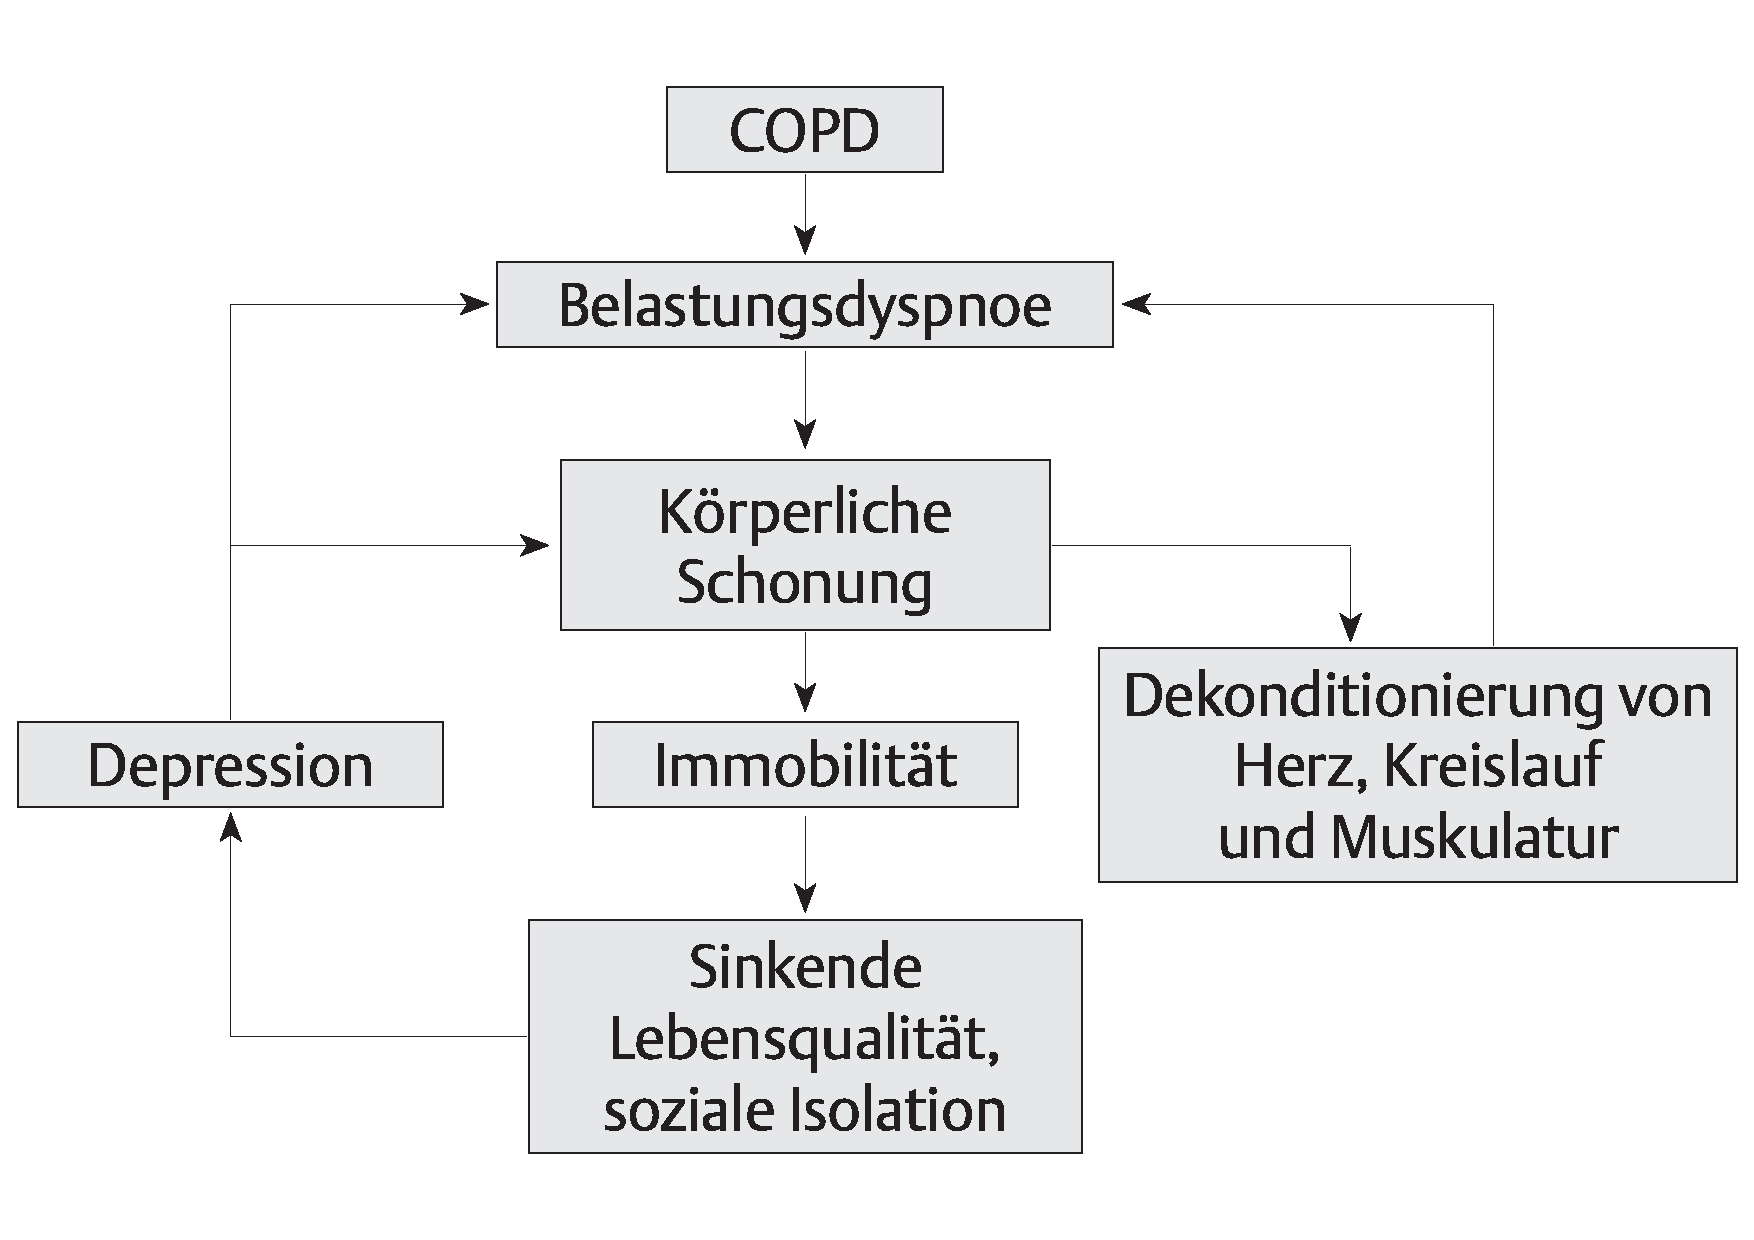
\includegraphics[width=0.6\textwidth]{teufelskreis}
  \caption{Circulus virtuosus, übernommen aus \cite[e19]{vogelmeier2007}}
  \label{fig:copd_teufelskreis}
\end{figure}

Die Angaben zur Prävalenz von Angst und Depression bei COPD variieren sehr. „Generalisierte Angststörungen werden in einer Häufigkeit von 2-16\%, Panikstörungen von 8-67\%, depressive Symptome und Depressionen zwischen 11 und 80\% sowie Angstsymptome in einem Bereich von 10-75\% angegeben“  \autocite[34]{kenn2011}.

An diesen Zahlen lässt sich erkennen, dass exakte Ergebnisse in Bezug auf die Prävalenz noch fehlen. Kenn und Kühl gehen davon aus, dass methodisch verschiedene Diagnoseansätze hierfür verantwortlich sind, wobei sie hierbei Ergebnisse aus Interviews, die sich an den Kriterien für psychische Störungen z.B. nach der ICD 10 orientieren, und Fragebögen gegenüberstellen. Generell erschwerten wohl neben den unterschiedlichen Erhebungsinstrumenten auch die Heterogenität der untersuchten Patientenkohorte mit verschiedenen Schweregraden die Interpretation der Ergebnisse \autocite[vgl.][35]{kenn2011}.
Zudem geben die Studienergebnisse keine Auskunft darüber, in wie weit bei Patienten, die eine COPD aufgrund eines längeren Nikotinabusus‘ entwickelt haben, bereits eine größere psychische Vulnerabilität und somit ein erhöhtes Risiko für die Ausbildung einer Depression oder Angst-/Panikstörung besteht. 

Ein evtl. wichtiges Konzept für den Krankheitsverlauf der COPD in seinen unterschiedlichen Facetten scheint die s.g. „Fear Avoidance" zu sein. Viele Patienten berichten von Angst vor auftretender Atemnot. Fear Avoidance- Konzept meint „die Angst vor der Verstärkung eines Krankheitssymptoms bzw. Verschlechterung des Verlaufs und daraus folgende Aktivitätsvermeidung" \autocite[111]{stenzel2013}. Dieses Konzept wurde jedoch bisher für COPD noch kaum diskutiert und erforscht. Eine neuere Studie zeigte jedoch, dass Fear Avoidance tatsächlich als Mediator des Zusammenhangs zwischen COPD-Status und Lebensqualität bzw. Gesundheitsstatus gesehen werden kann. Die Autoren plädieren daher dafür, dass im Rahmen der pneumologischen Rehabilitation auch psychotherapeutische Interventionen implementiert werden sollten, welche diesen Aspekt aufgreifen \autocite[112]{stenzel2013}. 

In dem später dargestellten musiktherapeutischen Konzept wird dieser Aspekt ebenfalls implizit aufgenommen werden. Durch achtsames Wahrnehmen eigener Grenzen und Möglichkeiten, aber auch durch übungszentriertes Arbeiten entwickeln die Patienten durch positive Erfahrungen im Zusammenhang mit Selbstregulation wieder mehr Selbstvertrauen und erleben sich als selbstwirksame Individuen, die sich nicht der auftretenden Atemnot ausgeliefert fühlen müssen.

In Studien wurde zudem ein signifikanter Zusammenhang zwischen einer erhöhten Mortalität und einer COPD mit begleitender depressiver oder Angstsymptomatik nachgewiesen. Aber auch in Bezug auf die Exazerbations- und Rehospitalisationsrate sowie die Leistungsfähigkeit und -bereitschaft von COPD-Patienten scheint hier die Ausbildung der genannten psychischen Erkrankung einen relevanten negativen Faktor darzustellen\autocite[vgl.]{kenn2011}.

Obgleich das zuvor Erläuterte heutzutage unter allgemeinmedizinischen und pneumologischen Fachärzten als bekannt anzunehmen ist, wird die Problematik in den Arzt-Patient-Gesprächen oftmals nicht thematisiert. Eine amerikanische Studie zeigte diese Diskrepanz zwischen der Prävalenz und Behandlungshäufigkeit psychischer Erkrankungen bei gleichzeitiger COPD. In einer Telefonumfrage von 1334 Patienten lagen bei 61\% psychische Auffälligkeiten, insbesondere Angstsymptome, vor. Lediglich 31\% dieser Patienten wurden diesbezüglich behandelt \autocite[vgl.][156]{fischer2007}.


\section{Zusammenfassende Betrachtung}
\label{zusammenfassende betrachtung}
Die vorherigen Ausführungen machen deutlich, um welch komplexes und schwerwiegendes Krankheitsbild es sich bei der COPD handelt. 

% ---------------------------------------------------------------------------
% ----------------------- end of thesis sub-document ------------------------
\newpage\thispagestyle{empty}
% this file is called up by thesis.tex
% content in this file will be fed into the main document

%: ----------------------- introduction file header -----------------------
\chapter{Musiktherapeutische Stimmarbeit}
\label{chapter:musiktherapeutische_stimmarbeit}
\setlength{\epigraphwidth}{8.0cm}
\epigraph{Singen als Ausdruck von Gefühl, Gedanken und Identität, als Bewältigung und soziale Aktivität, die Fühlen und Denken synchronisiert und Gemeinschaftsgefühl, Nähe und Zugehörigkeitsgefühl erzeugt, ist ein Kommunikationsmedium, das von frühester Kindheit bis in die letzten Lebensphasen des Menschen eine besondere Rolle spielt.}{Heiner Gembris} todo Fußnote Gembris 2008 S. 12
\ifpdf
    \graphicspath{{3_musiktherapeutische_stimmarbeit/figures/PNG/}{3_musiktherapeutische_stimmarbeit/figures/PDF/}{3_musiktherapeutische_stimmarbeit/figures/}}
\else
    \graphicspath{{3_musiktherapeutische_stimmarbeit/figures/EPS/}{3_musiktherapeutische_stimmarbeit/figures/}}
\fi
% ----------------------------------------------------------------------
%: ----------------------- introduction content -----------------------
% ----------------------------------------------------------------------
\lettrine{I}{n} diesem Zitat wird in knapper, jedoch prägnanter Form zusammengefasst, wie wichtig und wertvoll der stimmliche Ausdruck für den Menschen ist. In den folgenden Kapiteln soll das hier Skizzierte ausgeführt und -geweitet werden, um einen Eindruck für die Möglichkeiten der Stimmarbeit im musiktherapeutischen Kontext zu vermitteln.

Bevor im Folgenden selbstverständlich mit dem Begriff der "Stimme" umgegangen wird, scheint es sinnvoll, eine kleine Einführung in die Physiologie des Stimmapparats zu geben, um zum Einen die Komplexität der Funktionsweise unseres körpereigenen Instruments zu verstehen und um zum Anderen eine gemeinsame Grundlage für die Ausführungen in den nun folgenden Kapiteln zu schaffen. 

Die Stimmerzeugung basiert auf dem Zusammenspiel zwischen Körper, Atem und Stimmapparat (Kehlkopf und Ansatzrohr). Atem und Kehlkopffunktionen sind abhängig von dem Zusammenspiel und dem Spannungszustand der Muskeln. Haben wir beispielsweise aufgrund eines plötzlich auftretenden angstauslösenden Ereignisses einen erhöhten Körpertonus, so wird dies zwangsweise dazu führen, dass wir nicht mehr entspannt ein- und ausatmen, da sich die erhöhte Anspannung auch auf unsere Atemmuskulatur, insbesondere dem Zwerchfell als wichtigstem und größtem Atemmuskel überträgt. 

Für die Stimmerzeugung sind verschiedene Faktoren wichtig, die jedoch nicht einzeln nebeneinander stehen, sondern vielmehr ineinander übergreifen. 

Bevor es zu einer stimmlichen Äußerung kommt, bedarf es des Einfließens der Luft in die unteren Atemwege, die Lunge. Die Atmung als lebensnotwendiger Prozess wird über das Vegetativum gesteuert, das heißt, sie erfolgt nicht willentlich gelenkt; auf die Atmung im Speziellen wird unter Kapitel 3.2.5 näher eingegangen. Die Atemluft strömt für normal durch die sich im Kehlkopf befindenden und in Dreicksform geöffneten Stimmlippen. Kommt es nun zu einer stimmlichen Äußerung, schließt sich im ersten Schritt die Glottis, auch Stimmritze genannt, nach vollendetem Einatmen. Anschließend wird durch den nun folgenden Ausatem ein Überdruck auf die geschloßenen Stimmlippen erzeugt, welcher diese in Schwingung versetzt.
Für die Stimmerzeugung nun bedarf es des Ausatemstroms, welcher einen Überdruck erzeugt, der wiederum auf die Glottis, die s.g. Stimmritze, wirkt und sie kraftvoll öffnet. 
Stimmphysiologische Hintergründe todo

In den folgenden Kapiteln wird 

\section{Geschichtliche Einführung in das Thema}
Zu Beginn der weiteren Ausführungen in diesem Kapitel sollte der Blick auf den Gebrauch der Singstimme in der Gesellschaft gewendet werden, um ein klareres Gesamtbild dieses Themas entstehen lassen zu können.

Während das Singen in unserer Großelterngeneration noch weit verbreitet war, man beachte unseren großen Umfang an deutschem Liedgut, so hat die nationalsozialistisch geprägte Zeit der 30er und 40er Jahre einen Keil in diesen selbstverständlichen Gebrauch der Singstimme in Gemeinschaft getrieben.
Die Verschandelung deutschen Liedguts mit nationalsozialistischem Gedankengut und den Einsatz desgleichen für propagandistische Zwecke, sowie im Besonderen in der Jugendmusikbewegung der damaligen Zeit geschehen, führte u.a. zu "der späteren Voreingenommenheit gegenüber gemeinsamem Singen im Allgemeinen und gegenüber dem deutschen Volkslied im Speziellen" \autocite[9]{wolf2012}.

Hinzu kommt seitdem die Entwicklung neuer Medien und die Möglichkeit eines geöffneten Zugangs zu diesen. Laut Wolf hat dies großen Einfluss auf "die Entwicklung hin zu einer Vereinzelung der Menschen und hin zu einer Veränderung des menschlichen Alltagverhaltens" \autocite[10]{wolf2012}, wodurch die Notwendigkeit der gemeinschaftlichen Freizeitgestaltung, welche in früheren Zeiten oftmals das gemeinsame Singen beinhaltete, nachließ. Nur an vereinzelten Schauplätzen wie z.B. im Gottesdienst, im Stadion, bei den Pfadfindern oder in Chören wird das gemeinschaftliche Singen und/oder Grölen noch aktiv praktiziert.

In der MT war der Einsatz der Singstimme ebenfalls lange Zeit negativ konnotiert und wurde "[\ldots] als "Konflikt vermeidende Technik" in den heilpädagogisch orientierten Bereich der Kindermusiktherapie oder das palliativ orientierte Feld der Geriatrie verortet" \autocite[10]{wolf2012}. So war das Singen von Liedern im Rahmen einer "psychotherapeutisch orientierten MT" lange Zeit ausgeklammert. Zudem wurde die Stimme zum klanglichen Ausdruck kaum genutzt, da man einen zu großen Widerstand seitens der Patienten erwartete (siehe weiter unten in diesem Kapitel). 

Durch den sich in den letzten Jahren vollziehenden Paradigmenwechsel in der psychotherapeutischen Behandlung im Allgemeinen und der musiktherapeutischen im Speziellen von einem eher konfliktzentrierten Ansatz und dem Konzept der Katharsis hin zu einem eher ressourcenorientierten und stabilisierenden Arbeiten veränderte sich auch die Einstellung gegenüber dem Singen\autocite[vgl.][11]{wolf2012}. Einer kleinen Forschergruppe aus Musiktherapeuten und -pädagogen, aber auch bekannten Ärzten (wie z.B. Dr. Gerald Hüther, Dr. Manfred Spitzer u.a.) ist es zu verdanken, dass wir heute mehr über die Wirkung des Singens auf Körper, Geist und Seele wissen. Sie waren es, die zu einer Etablierung von Singgruppenarbeit primär beigetragen haben. Im klinischen Bereich hat sich insbesondere der Musiktherapeut Wolfgang Bossinger verdient gemacht und eine mittlerweile über Deutschland verbreitete Initiative, "Singende Krankenhäuser", ins Leben gerufen. Aber auch Sabine Rittner und Karl Adamek haben zu einem großen Erkenntnisgewinn und möglichen Vorgehensweisen in diesem Bereich verholfen.

\section{Einsatz der (Sing-)Stimme im musiktherapeutischen Kontext}

Heute wird die (Sing-)Stimme im psychotherapeutischen Kontext in unterschiedlicher Art und Weise eingesetzt, genutzt und betrachtet. Sabine Rittner \autocite[vgl.][204 ff.]{rittner2008} hat diese Bereiche kategorisiert, um ihre Komplexität zu entzerren. Diese insgesamt acht Kategorien fließen zum Teil in die folgenden Ausführungen ein: 
Stimme als\ldots
\begin{enumerate}
\item Medium der verbalen und nonverbalen Beziehungsgestaltung
\item Methode in der körperorientierten Musikpsychotherapie
\item Diagnostikum im therapeutischen Gespräch
\item Indikator für die therapeutische Übertragung- und Gegenübertragung
\item Symptom
\item Ausdrucksmittel
\item Selbstheilungs-Mittel
\item Medium zur Tranceinduktion
\end{enumerate}

Bereits im Mutterleib beginnt der Beziehungsaufbau zwischen Mutter und Kind über stimmliche Äußerung. Ab der 23. Schwangerschaftswoche kann der Fötus seine Umwelt auditiv wahrnehmen und auf sie reagieren. Die Stimme der Mutter tritt dabei in den Vordergrund. Wie man durch Untersuchungen kurz nach der Geburt festgestellt hat, können Säuglinge die Stimme ihrer Mutter von der anderer Personen unterscheiden \autocite [vgl.][22f]{noecker-ribeaupierre2004}. 

Die stimmliche Äußerung ist für die Entwicklung des Kindes von besonderer Bedeutung: durch Abstimmungsprozesse mit den primären Bezugspersonen auf unterschiedlichen sensorischen Ebenen, insbesondere durch stimmliche Interaktion, lernt es, die Welt und sich über die s.g. amodale Wahrnehmung zu begreifen. Gerade in dieser Zeit wird deutlich, welche Bedeutung die Stimme im Hinblick auf die Mitteilung der eigenen emotionalen Gestimmtheit hat, wie sich Beziehung ohne Worte aber dennoch durch stimmlichen Ausdruck gestalten lässt. Insbesondere durch den Einsatz von Vokalen kann diese "emotionale Tönung" \autocite[205]{rittner2008} deutlich werden, wie weiter unten näher erläutert wird.

Rittner \autocite [vgl.][106f.]{rittner1990} betont zudem die therapeutische Relevanz der Polaritäten, die sich im Schreien und Lallen des Säuglings äußern. Mit dem ersten Schrei tritt der Säugling zum ersten Mal geräuschvoll mit seiner neuen/ alten Umwelt in Kontakt und entlädt dabei die zuvor im ersten Einatem aufgebaute Anspannung. Diese Form der Kontaktaufnahme mit der Außenwelt differenziere sich, so Rittner, in den darauffolgenden Wochen immer mehr zu einem "gerichteten Appell" in Bezug auf die Befriedigung der Grundbedürfnisse. Im Lallen hingegen zeige der Säugling aus einer befriedigten Grundstimmung heraus eine "lustbetonte, nach innen gerichtete, autoerotisch-regressive Handlung", die oftmals unterbrochen wird, sobald beispielsweise im Außen Geräusche auftreten oder eine Person das Zimmer betritt und ihn so aus seiner Versunkenheit herauszieht. 
Die o.g. Polaritäten können aus diesen beiden Handlungen heraus folgendermaßen beschrieben werden: "die Verbindung zwischen Innenraum und Außenraum, zwischen Regression, dem wohligen Sich-Einhüllen, und Progression, in der sich lebenserhaltende aggressive Anteile artikulieren" \autocite[vgl.][106f.]{rittner1990}.

Diese Aspekte sind wesentlich für die Gestaltung und die Arbeit im Rahmen einer therapeutischen Beziehung. Mithilfe musiktherapeutischer Stimmarbeit ist es uns somit möglich, in sehr direkter Form an diese sehr frühen Erfahrungswelten anzuknüpfen und an einer Ausbalancierung der o.g. Polaritäten zu arbeiten. 

Allerdings gilt es dabei u.a. zu beachten, dass der Mensch im Laufe seiner Entwicklung Hemmungsmechanismen ausbildet, welche auf die Sauberkeitserziehung sowie auf Sozialisationsprozesse zurückzuführen sind. Diese Mechanismen lassen sich gliedern in "Scham- und Peinlichkeitsgefühle als auch [in] psychische Instanzen, die das Gewissen und Schuldgefühle auslösen" \autocite [106f.]{rittner1990}. 

Durch das Singen kommen wir, wie bereits zuvor dargelegt, schnell in Kontakt mit unserer primär unbewussten Gefühlswelt. Aufgrund der Nähe zu "frühkindlichen Gefühlszuständen vor der Schamhemmung" (todo Klausmeier zitiert in Rittner 1990 todo) und damit einem sehr intensiven emotionalen Erleben kann der unvorbereitete Einsatz der Singstimme überflutend und angstauslösend hinsichtlich des ungewollten Zeigens von u.a. abgewehrten Selbstanteilen wirken. 

Da das Thema Scham m.E. wichtig ist für die Arbeit mit der Stimme im musiktherapeutischen Rahmen und bereits am Anfang dieses Kapitels in Wolfs Aussage zu Widerständen in diesem Kontext anklingt, soll an dieser Stelle darauf eingegangen werden.

\subsection{Scham und Stimme}
Zunächst eine kurze Erläuterung des Begriffs. Unter dem Titel "Scham. Lautloses Tönen" erschien 2012 ein Themenheft der Musiktherapeutischen Umschau (MU). Hierin beschrieb Tilman Weber in knapper Form und aus unterschiedlichen theoretischen Perspektiven die "Scham" folgendermaßen:
"Vielleicht kann man sagen, dass Scham aus triebpsychologischer Sicht einem typischen Es - Überich - Konflikt entspringt, aus objektpsychologischer Sicht der Diskrepanz zwischen Individuum und Gesellschaft und aus ichpsychologischer Sicht der Differenz zwischen Anspruch und Vermögen" \autocite[215]{weber2012}. 

Tiedemann, tiefenpsychologischer und analytischer Psychotherapeut und Forscher, beschreibt Scham als einen Vorgang, in dem "das Subjekt eine Infragestellung und Bedrohung der sozialen Wertschätzung, Akzeptanz und Anerkennung" \autocite[219]{tiedemann2012} erlebt. Daher tritt sie meist in solchen Situationen auf, in denen ein "Mensch etwas Intimes preisgibt" \autocite[219]{tiedemann2012}. 

Die Stimme ist das intimste körpereigene Instrument des Menschen. Jede stimmliche Äußerung gibt ein Stück unserer individuellen Ge-stimmt-heit preis. An unterschiedlichen Stellen in der hierzu relevanten Literatur wurde immer wieder darauf hingewiesen, dass eine stimmliche Maskierung des eigenen affektiven Zustandes nicht möglich ist \autocite[vgl.][279]{decker-voigt1992} \autocite[vgl.][481]{rittner2009a}. Je nach Stellung der Stimmknörpelchen und des Tonus der über 100 an der stimmlichen Äußerung beteiligten Muskeln \autocite[vgl.][40]{cramer1998} gestaltet sich das nach außen Dringende. Denn jegliches Zurückhalten oder Verdecken von aufkeimenden Emotionen führt zu Störungen der Feinabstimmung innerhalb des Stimmapparates. Dies kann zu Muskelverspannungen führen, die wiederum in der erklingenden Stimme durch einen harten Stimmansatz, verhauchen der Stimme durch nicht zu Klang gewordener herausströmender Luft, eine höhere oder tiefere Stimmfrequenz u.a. zu hören sind \autocite[vgl.][279]{decker-voigt1992}. 
Laut Rittner vernehmen wir die "emotionale Tönung" der Person durch die Prosodie [=das, was dazu singt). Insbesondere durch den Klang der Vokale, welche physikalisch betrachtet als Klangträger gleichmäßige Schwingungsmuster, Konsonanten hingegen als Geräuschträger ungleichmäßige Schwingungswellen erzeugen, erfahren wir im Sinne der oben genannten physiologischen Vorgänge etwas über die Gestimmtheit unseres Gegenübers. Dabei kommt dem Singen eine besondere Rolle zu: "Singen unterscheidet sich vom Sprechen dadurch, dass der klanglich-nonverbale Schwingungsanteil der emotionalen Botschaft durch die Verlängerung der Vokale im ausgedehnten Ausatem deutlich in den Vordergrund tritt" \autocite[205]{rittner2008}.

Die vorherigen Ausführungen machen deutlich, dass es sich bei der gesanglichen Äußerung um ein sehr unmittelbares und intimes Zeigen der emotionalen Verfassung handelt. Die stimmliche Äußerung ist direkter als das Spielen eines Musikinstruments, welches bereits räumlich von uns getrennt ist und evtl. sogar einen Schutz bietet i.S. eines sich dahinter Verstecken-Könnens. Wenn wir also im musiktherapeutischen Kontext mit der Singstimme arbeiten, sollten wir uns dieser unmittelbaren Verbindung bewusst sein. Denn das Singen, vorallem in der Improvisation, welche häufig mit der Sorge um Kontrollverlust verbunden ist, kann als "zu starker emotionaler Ausdruck abgewehrt und blockiert werden" \autocite[485]{rittner2009a}. Um jedoch der Abwehr aus Scham entgegen zu wirken, sei es laut Rittner wichtig, stimmliche Interventionen im Verlauf der musiktherapeutischen Behandlung methodisch anzubahnen. So könne beispielsweise mit bekannten, durchkomponierten Liedern, Melodien und Rhythmen begonnen werden, um sich der ursprünglichen stimmlichen, improvisierenden Äußerung, wie sie zu Beginn des Lebens wertfrei bestand, zu nähern. 

\subsection{Diagnostische Überlegungen}
Im Rahmen der Diagnostik gibt die Stimme des Patienten bereits wichtige Hinweise auf dessen aktuelle Befindlichkeit sowie seine Stimmung. Durch aufmerksames Hinhören kann erspürt werden, ob das Gesagte in sich "stimmig", sprich kongruent ist. Zudem gibt sie bereits Auskunft über den biografischen Hintergrund der sich äußernden Person, denn sie hat sich mit unseren über die Zeit gesammelten Lebenserfahrungen weiterentwickelt und diese in sich aufgesogen. So gilt die Stimme unter Experten als "Klingendes Hologramm der Persönlichkeit" \autocite{adamek1999}, "lauthafte Biographie" \autocite{gundermann1994} und bei Rittner erfahren wir über den Klang der Stimme etwas über die "leib-seelische Gewordenheit" \autocite[211]{rittner2008} des Menschen.
Dabei scheint jedoch nicht so sehr der Inhalt des Gesagten aufschlussreich, sondern vielmehr der "Klang der Stimme (Klangspektrum, Modulation, Lautstärkeänderungen, Stimmsitz, Vokaleinsatz etc.), die Sprechweise (Artikulation, Phrasierung, Pausensetzung etc.) und die Atmung (Atemfrequenz, Atemtiefe, hörbares Einatmen, Sitz des Atemraumes im Körper etc.)" als auch "die Art der Gestaltung von Sprechpausen, Abbrüchen, Momenten des Innehaltens, Verzögerungen u.ä." \autocite[210]{rittner2008}. Diese stillen Momente vertiefen jedoch oftmals das atmosphärische Wahrnehmen und können zu einem tieferen Verstehen ohne Ablenkung führen. 
Gerade in Momenten der Inkongruenz von Semantik, Prosodie, Mimik, Gestik etc. wurde festgestellt, dass der Zuhörer sich in diesem Falle weniger auf den Inhalt des Gesprochenen seines Gegenübers bezieht, sondern in einen visuell-auditiven Modus wechselt, in welchem die Semantik in den Hintergrund rückt \autocite [vgl.][206f.]{rittner2008}.

\subsection{Weitere Aspekte musiktherapeutischen Arbeitens mit der Stimme}
Rittner

\subsection{Vokalimprovisation}
Die Vokalimprovisation ist eine sehr spielerische Möglichkeit, die Stimme in die musiktherapeutische Arbeit einzubeziehen. Sie gilt als der "Einsatz des gesamten Ausdrucksspektrums stimmhafter wie stimmloser Äußerungen, meist im Schutz einer Gruppe mit oder ohne Themenvorgabe" \autocite [108]{rittner1990}. Dabei sei sie stets gebunden an persönliche, situative, musikalisch oder symbolische Inhalte und verfolge therapeutische, pädagogische oder musikalisch-künstlerische Ziele \autocite [109]{rittner1990}.


\subsection{Die Wichtigkeit des Einbezugs von Körper und Atem in dieser Arbeitsweise}
Ilse Middendorf
Schlaffhorst Andersen
MT und Atem (Buch)
Annette Cramer
Rittner
Hertha Richter

\section{Die Wirkung des Singens auf Körper und Psyche} 
Bossinger, Adamek und Cramer
Selbstheilungskräfte





\newpage\thispagestyle{empty}
% ----------------------------------------------------------------------
\chapter{Andere wichtige therapeutische Ansaetze für die Arbeit mit COPD Patienten}
\label{chapter:andere_wichtige_therapeutische_ansaetze_für_die_arbeit_mit_copd_patienten}
%put your favorite quote
\epigraph{Choose a job you love, and you will never have to work a day in your life.}{Confucius}

% the code below specifies where the figures are stored
\ifpdf
    \graphicspath{{4_segmentation/figures/PNG/}{4_andere_wichtige_therapeutische_ansaetze_für_die_arbeit_mit_copd_patienten/figures/PDF/}{4_andere_wichtige_therapeutische_ansaetze_für_die_arbeit_mit_copd_patienten/figures/}}
\else
    \graphicspath{{4_andere_wichtige_therapeutische_ansaetze_für_die_arbeit_mit_copd_patienten/figures/EPS/}{4_andere_wichtige_therapeutische_ansaetze_für_die_arbeit_mit_copd_patienten/figures/}}
\fi

\lettrine{T}{his} chapter 


georef!
% this file is called up by thesis.tex
% content in this file will be fed into the main document

%: ----------------------- name of chapter  -------------------------
\chapter{Konzept}
\label{chapter:konzept}
\setlength{\epigraphwidth}{7.0cm}
\epigraph{To study and not think is a waste. To think and not study is dangerous.}{Confucius}

\section{Gedanken zu COPD und Singen}
Wenngleich der Einsatz der (Sing-)Stimme insbesondere im Hinblick auf ein bewussteres und verlängertes (Aus-)Atmen m.E. in diesem Bereich sehr sinnvoll erscheint, so ist gleichzeitig auch Vorsicht geboten. In diesem Bereich kann es zu entzündlichen Vorgängen rund um den Stimmapparat aufgrund der medikamentösen Behandlung und einer geschwächten Immunabwehr kommen. In diesen Fällen ist es notwendig, durch einen Phoniater abklären zu lassen, ob die Stimme der Schonung bedarf oder aber der gezielte und bedachte Einsatz der Stimme zu einer Besserung der Stimmfähigkeit beiträgt \autocite[vgl.][103ff.]{alavi2009}.
%: ----------------------- paths to graphics ------------------------
% change according to folder and file names
\ifpdf
    \graphicspath{{5_konzept/figures/PNG/}{5_konzept/figures/PDF/}{5_konzept/figures/}}
\else
    \graphicspath{{5_konzept/figures/EPS/}{5_konzept/figures/}}
\fi

\lettrine{T}{he} algorithm for

\newpage\thispagestyle{empty}
% ---------------------------------------------------------------------------
%: ----------------------- end of thesis sub-document ------------------------
% ---------------------------------------------------------------------------
%% this file is called up by thesis.tex
% content in this file will be fed into the main document

%: ----------------------- name of chapter  -------------------------
\chapter{Auswertung eigener Erfahrungen und Aufzeichnungen aus der Umsetzungsphase}
\label{chapter:auswertung_eigener_erfahrungen_und_aufzeichnungen_aus_der_umsetzungsphase}
\setlength{\epigraphwidth}{7.0cm}
\epigraph{By three methods we may learn wisdom: First, by reflection, which is noblest; second, by imitation, which is easiest; and third by experience, which is the bitterest.}{Confucius}

% change according to folder and file names
\ifpdf
    \graphicspath{{6_auswertung_eigener_erfahrungen_und_aufzeichnungen_aus_der_umsetzungsphase/figures/PNG/}{6_auswertung_eigener_erfahrungen_und_aufzeichnungen_aus_der_umsetzungsphase/figures/PDF/}{6_auswertung_eigener_erfahrungen_und_aufzeichnungen_aus_der_umsetzungsphase/figures/}}
\else
    \graphicspath{{6_auswertung_eigener_erfahrungen_und_aufzeichnungen_aus_der_umsetzungsphase/figures/EPS/}{6_auswertung_eigener_erfahrungen_und_aufzeichnungen_aus_der_umsetzungsphase/figures/}}
\fi

\lettrine{A}{s} input, the path planner requires the UAV's current position, the sparse collider cloud and a list of waypoints.



\chapter{Motion Control for Autonomous Flight}
\label{section_motion_control_for_autonomous_flight}

Multirotor UAVs require 

\newpage\thispagestyle{empty}
% ---------------------------------------------------------------------------
%: ----------------------- end of thesis sub-document ------------------------
% ---------------------------------------------------------------------------
%\chapter{Abschließende Betrachtung} % top level followed by section, subsection

\setlength{\epigraphwidth}{7.5cm}
\epigraph{Study the past, if you would divine the future.}{Confucius}

\ifpdf
    \graphicspath{{X/figures/PNG/}{X/figures/PDF/}{X/figures/}}
\else
    \graphicspath{{X/figures/EPS/}{X/figures/}}
\fi

\lettrine{T}{his} dissertation 

\newpage\thispagestyle{empty}
% ---------------------------------------------------------------------------
%: ----------------------- end of thesis sub-document ------------------------
% ---------------------------------------------------------------------------



% --------------------------------------------------------------
%:                  BACK MATTER: appendices, refs,..
% --------------------------------------------------------------

% the back matter: appendix and references close the thesis
% this file is called up by thesis.tex
% content in this file will be fed into the main document

%: ----------------------- name of chapter  -------------------------
%\appendix
\phantomsection
\renewcommand{\chaptername}{Appendix} % uncomment to print only "1" not "Chapter 1"
\renewcommand\thechapter{\Alph{chapter}}
\setcounter{chapter}{0}
%\appendix
\chapter{Source code, datasets, and videos} % top level followed by section, subsection
\label{chapter:appendix}


%: ----------------------- paths to graphics ------------------------

% change according to folder and file names
\ifpdf
    \graphicspath{{X/figures/PNG/}{X/figures/PDF/}{X/figures/}}
\else
    \graphicspath{{X/figures/EPS/}{X/figures/}}
\fi

%: ----------------------- contents from here ------------------------
\begin{sloppypar}
\lettrine{T}{he} source code for all proposed algorithms in this dissertation, including 

\end{sloppypar}



\newpage\thispagestyle{empty}









% ---------------------------------------------------------------------------
%: ----------------------- end of thesis sub-document ------------------------
% ---------------------------------------------------------------------------



%: ----------------------- bibliography ------------------------

% The section below defines how references are listed and formatted
% The default below is 2 columns, small font, complete author names.
% Entries are also linked back to the page number in the text and to external URL if provided in the BibTex file.

% PhDbiblio-url2 = names small caps, title bold & hyperlinked, link to page
%\begin{multicols}{2} % \begin{multicols}{ # columns}[ header text][ space]
%\begin{tiny} % tiny(5) < scriptsize(7) < footnotesize(8) < small (9)



\printbibliography[]
%\bibliographystyle{Latex/Classes/PhDbiblio-url2} % Title is link if provided
%\begin{footnotesize}
%\bibliographystyle{alpha}
%\bibliographystyle{natbib}
%\renewcommand{\bibname}{Referenzen} % changes the header; default: Bibliography
%\bibliography{bibliography} % adjust this to fit your BibTex file
%\end{footnotesize}
%\end{tiny}
%\end{multicols}
\newpage\thispagestyle{empty}
%\chapter*{Eidesstattliche Versicherung} 

Hiermit erkl\"are ich an Eides statt, dass ich die vorliegende Dissertationsschrift selbst
verfasst und keine anderen als die angegebenen Quellen und Hilfsmittel benutzt habe.

\vspace{150pt}
\noindent Hamburg, den \hfill Unterschrift

\vspace{30pt}
\noindent \rule{\textwidth}{0.5pt}

% --------------------------------------------------------------
% Various bibliography styles exit. Replace above style as desired.

% in-text refs: (1) (1; 2)
% ref list: alphabetical; author(s) in small caps; initials last name; page(s)
%\bibliographystyle{Latex/Classes/PhDbiblio-case} % title forced lower case
%\bibliographystyle{Latex/Classes/PhDbiblio-bold} % title as in bibtex but bold
%\bibliographystyle{Latex/Classes/PhDbiblio-url} % bold + www link if provided

%\bibliographystyle{Latex/Classes/jmb} % calls style file jmb.bst
% in-text refs: author (year) without brackets
% ref list: alphabetical; author(s) in normal font; last name, initials; page(s)

%\bibliographystyle{plainnat} % calls style file plainnat.bst
% in-text refs: author (year) without brackets
% (this works with package natbib)

%: Declaration of originality

% Thesis statement of originality -------------------------------------

% Depending on the regulations of your faculty you may need a declaration like the one below. This specific one is from the medical faculty of the university of Dresden.

\begin{declaration}        %this creates the heading for the declaration page

I herewith declare that I have produced this paper without the prohibited assistance of third parties and without making use of aids other than those specified; notions taken over directly or indirectly from other sources have been identified as such. This paper has not previously been presented in identical or similar form to any other German or foreign examination board.

The thesis work was conducted from XXX to YYY under the supervision of PI at ZZZ.

\vspace{10mm}

CITY,

\end{declaration}


% ----------------------------------------------------------------------

\end{document}
